\chapter{Transformations of Energy}



\small

\begin{quote}
%Dieu a choisi celuy qui est... le plus simple en hypotheses et le plus riche 
%en phenomenes 
God has chosen that which is the most simple in 
hypotheses and the most rich in phenomena. (Leibniz, 
Discours de m\'etaphysique, VI, 1686)
\end{quote} 

%\begin{quote} The ordinary man (or woman) thinks he knows what time is
%but cannot say. The learned man, physicist or philosopher, is not sure
%he knows but is ready to write volumes on the subject of his
%speculation and ignorance. (David Landes in \emph{Revolution in Time} 1983)
%\end{quote}

\begin{quote}
The sight of day and night, and the months and the revolutions of the
years, have created number and have given us conception of time,
and the power of inquiring about the nature of the Universe. (Plato 
in \emph{Timaeus})
\end{quote}

\begin{quote}
... in a purely mechanical world, the tree could become a shoot 
and a seed again, the butterfly turn back into a caterpillar, and the
old man into a child. No explanation is given by the mechanistic doctrine
for the fact that it does not happen. (Ostwald)
\end{quote}

\begin{quote} ... a complete explanation of the arrow requires
explaining why the universe started out as it did. It is a problem
in cosmology. (Hawking)
\end{quote}
\normalsize

\section{Kinetic Energy and Heat Energy}

\emph{Thermodynamics} is fundamental in a wide range of phenomena from
macroscopic to microscopic scales. 
Thermodynamics essentially concerns the interplay between
\emph{kinetic energy} and  \emph{heat energy} in a \emph{gas} or \emph{fluid},
where heat energy is a form of small scale kinetic energy.
Thermodynamics thus concerns transformations between large scale
kinetic energy and small scale kinetic energy in the form of heat.
Large scale kinetic energy, or \emph{mechanical energy}, 
may generate heat energy by 
\emph{compression} or \emph{turbulent dissipation}. 
Heat energy may generate (large scale) kinetic energy by \emph{expansion}, but
not through a \emph{reverse} process of turbulent dissipation. 
Thermodynamics is closely connected to the dynamics of \emph{slightly viscous}
and \emph{compressible} gases, since substantial compression and 
expansion can occur in a gas, but less in fluids (and solids).

  
\section{Cosmology and Big Bang}

\emph{Cosmology} is the scientific study of the large scale properties of the 
\emph{Universe} as a whole, including its   
origin, evolution and ultimate fate. 
%The prevailing theory is 
%the so-called idea of a Big Bang where intense heat generated a lot
%of kinetic energy collected in galaxies of stars
%moving away from each other with velocity. 
The \emph{Big Bang} model postulates that 12 to 14 billion years ago,
the universe was in a very hot very dense 
state, which expanded along with galaxies and stars being 
formed by gravitation from variations in density, see Fig. \ref{bigbang}.
 It is believed that
we can see remnants of the hot 
dense matter as the now very cold cosmic microwave background radiation, 
which still pervades the universe as a slightly varying glow across 
the entire sky, see Fig. \ref{cobe}, a discovery made 
by the Cosmic Background Explorer COBE-telescope, which gave
the Nobel Prize in 2006 to John Mather and George Smoot.
Cosmology is basically a very (very) large scale application of thermodynamics
as an interplay of mass, momentum and energy governed by 
gravitational and inertial forces and driven by nuclear reactions.
% \begin{figure}[bhpt]
% \centerline{
% \includegraphics[height=8.0cm]{theoryoftimepict/bigbang.eps}
% }
% \caption{Thermodynamics of Big Bang from $10^{-41}$ seconds to 15 billion years.}
% \label{bigbang}
% \end{figure}   % --- removed: theoryoftimepict/bigbang.eps not in repo ---
\begin{figure}[bhpt] 
\centerline{ 
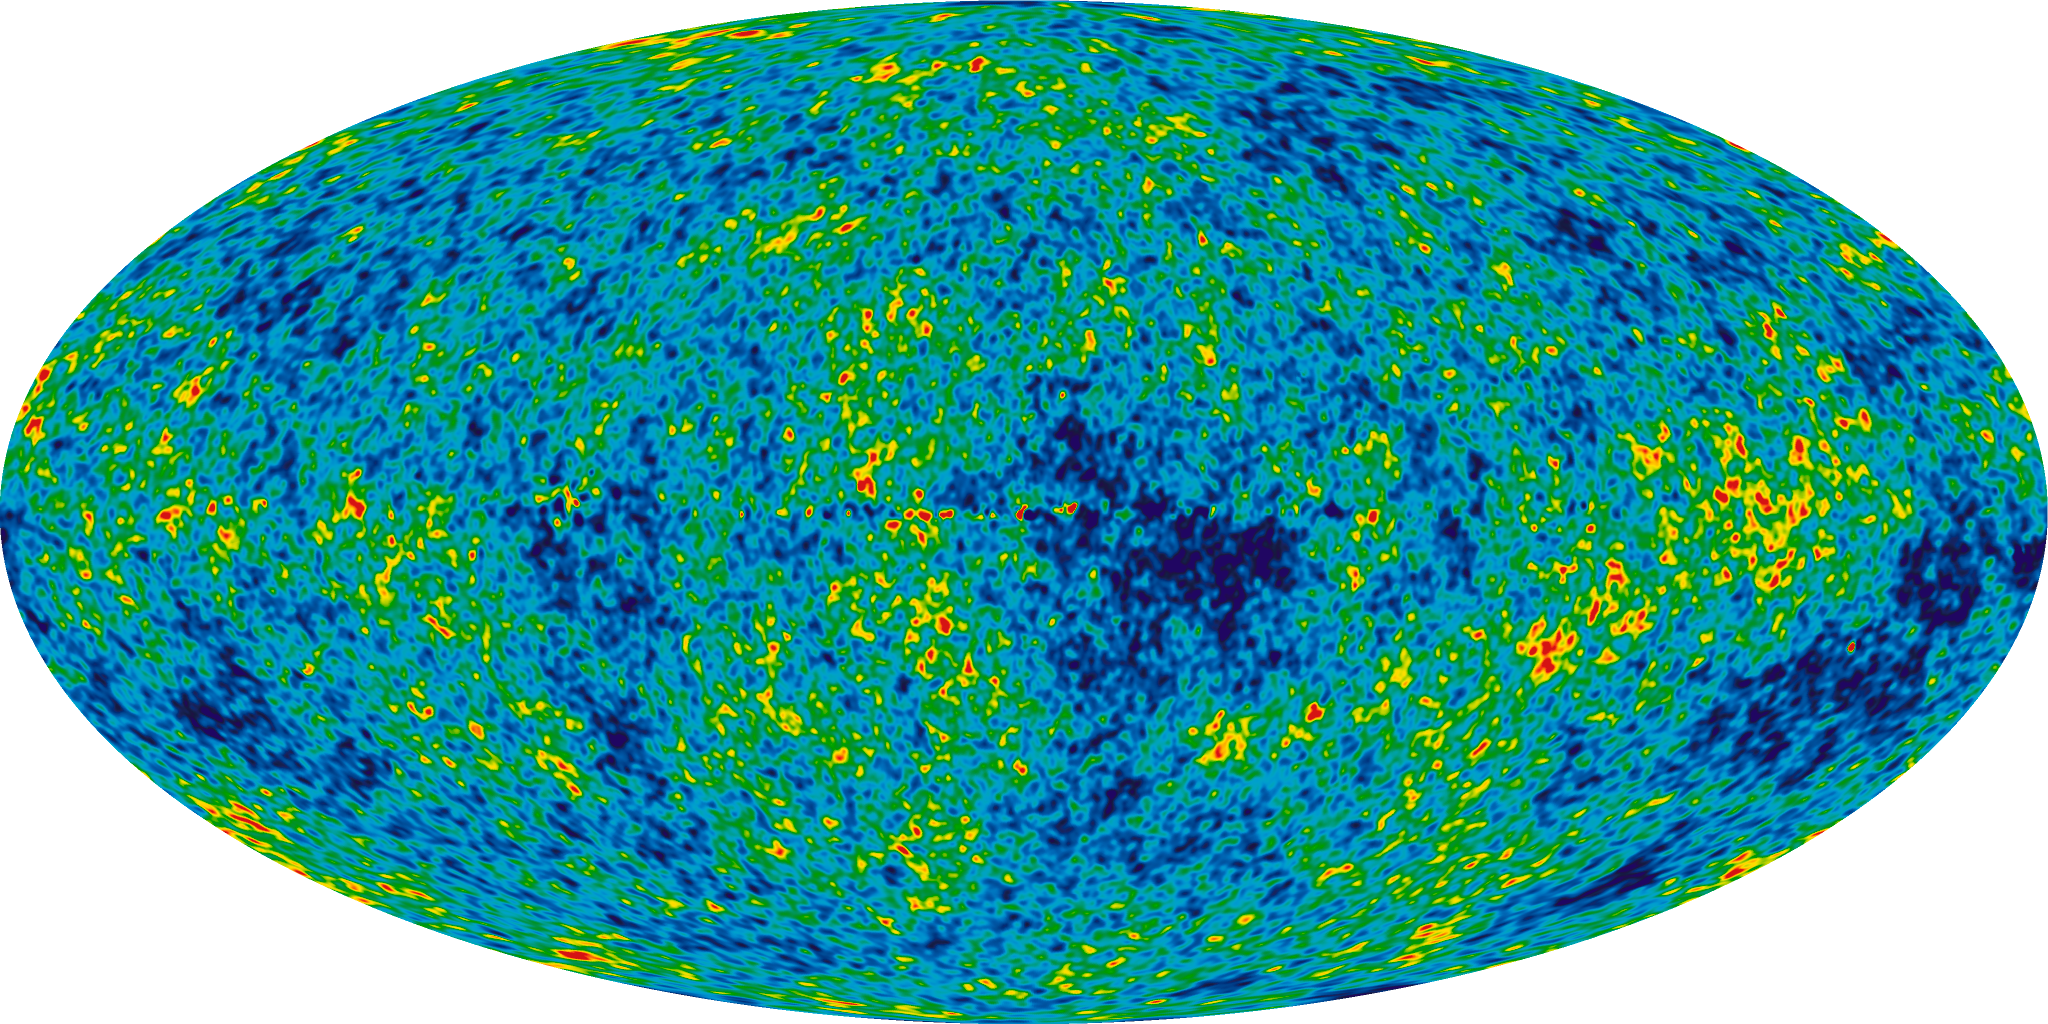
\includegraphics[height=4.0cm]{ambsthermopict/CMB_ILC_Map300.eps} 
} 
\caption{Cosmic back-ground radiation
according to COBE.}
\label{cobe} 
\end{figure}



%The Big Bang Model rests on the two theoretical pillars of
%Einstein's General Relativity and the Cosmological Principle.
%The key concept of General Relativity is that matter tells space how 
%to curve, and space tells matter how to move. 
%The Cosmological Principle states that matter in the universe is 
%homogeneous and isotropic when averaged over very large scales,
%supported by the observation that the cosmic microwave background 
%radiation has a temperature which 
%is highly uniform over the entire sky. 
%This fact strongly supports the notion that the gas which emitted this radiation 
%long ago was very uniformly distributed.

\section{Astronomy and Nuclear Energy}

The \emph{stars} were formed in the early Universe 
by accretion of mass by gravitational collaps 
increasing the temperature of a central core and thus igniting 
the star in a nuclear fusion process
with first deuterium and then hydrogen being transformed to helium under
intense release of energy (according to Einsteins famous
formula $E=mc^2$) increasing the pressure and counterbalancing
the gravitational collaps. \emph{Planets} may be formed 
from heavier atoms and molecules created in nuclear processes in stars,
and under favorable conditions give rise to (intelligent) \emph{life}
and theories of thermodynamics. 
Stars of 0.4-10 times the mass of our own Sun
expand into red giant very bright stars, when 
the supply of hydrogen in the core is empty and fusion starts in an 
outer core. Our own Sun thus eventually will swallow the Earth
into a fusion process, but this is estimated to be a couple of billion
years away. The thermodynamics of the Sun thus is the basis
of both life and death of the Earth.

% \begin{figure}[bhpt]
% \centerline{
% \includegraphics[height=8.0cm]{theoryoftimepict/impact.eps}
% }  % --- removed: theoryoftimepict/impact.eps not in repo; caption follows but unused ---
\iffalse
\begin{figure}[bhpt]
\centerline{
\includegraphics[height=8.0cm]{theoryoftimepict/impact.eps}
}
\caption{Asteroid impact on the surface of the Earth with irreversible transfer of large
scale kinetic energy
into small scale kinetic energy in the form of heat energy.}
\label{impact}
\end{figure}
\fi  % --- end removed impact.eps figure block ---



\section{Geology and Global Warming}
	
\emph{Geology} or earth science contains the subfields of
geophysics, glaciology, 
%petrology, seismology, 
volcanology, climatology and meteorology 
connecting to the the central issue of 
the thermodynamics of \emph{global warming}. Computational 
simulation of global climate change has a very important role to play
to find out what actions are beneficial for 
sustainable development and long-time survival. 



\begin{figure}[bhpt] 
\centerline{ 

\includegraphics[height=8.0cm]{ambsthermopict/earth.eps} 
} 
\caption{The Earth}
\label{nse_people} 
\end{figure}

\begin{figure}[bhpt] 
\centerline{ 
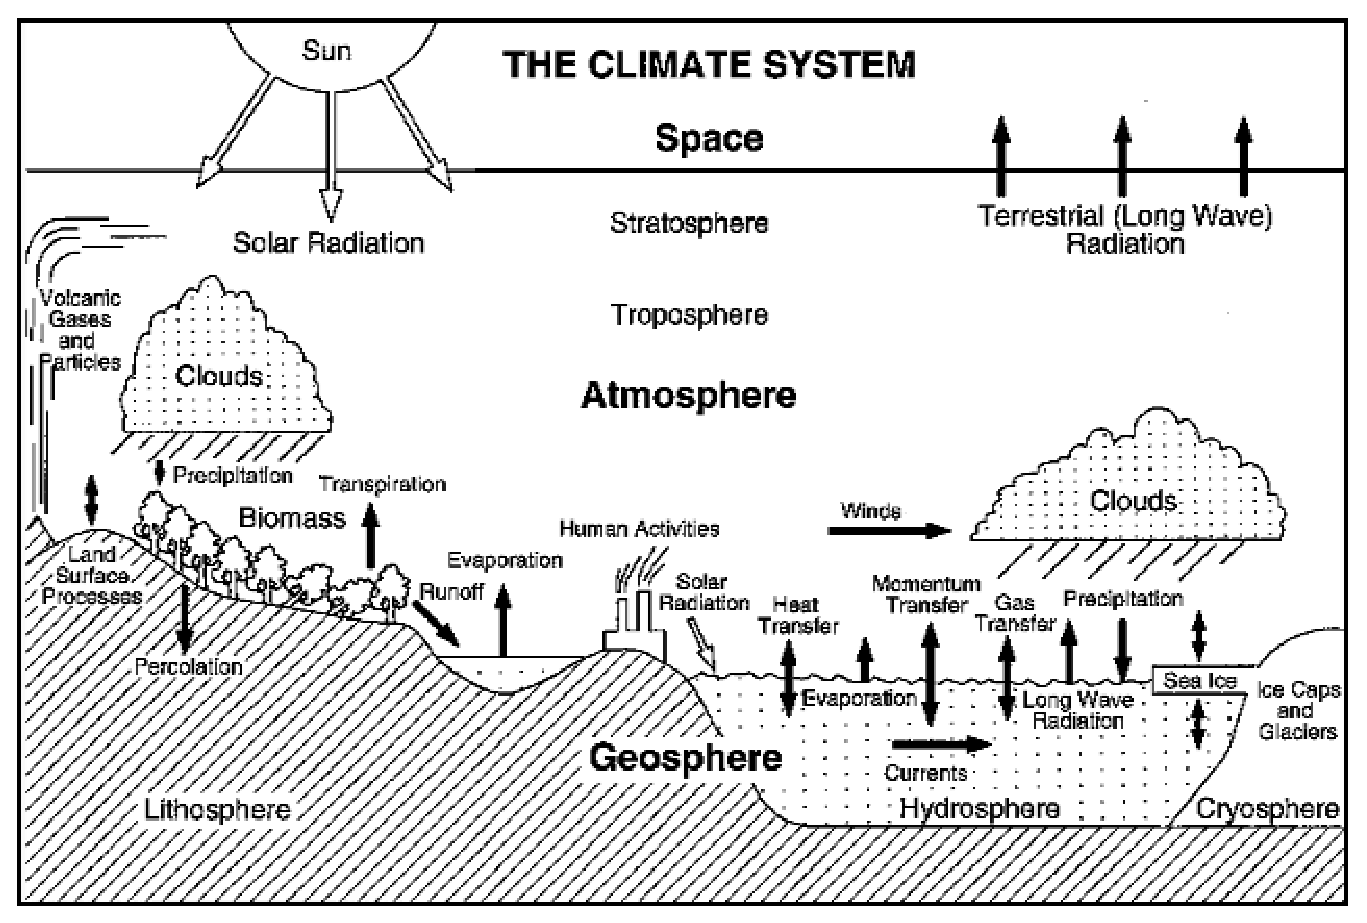
\includegraphics[height=6.0cm]{ambsthermopict/climate.eps} 
} 
\caption{Global heat balance.}
\label{nse_people} 
\end{figure}


\section{Black Body Radiation and the Sun}


A \emph{black body} absorbs incoming white light of all frequencies, 
from high frequency ultraviolet to low frequency infrared, but only radiates
low frequency light (with color depending on 
the temperature of the body).  This is the basis of the gross energy balance
of the Earth absorbing white light from the hot Sun and radiating 
low frequency light into empty space. One can view  
black body absorption/emission as an (irreversible) 
thermodynamic process transforming high frequency light energy  
to low frequency (long wave) light energy \cite{blackbody}. 


\begin{figure}[bhpt] 
\centerline{ 
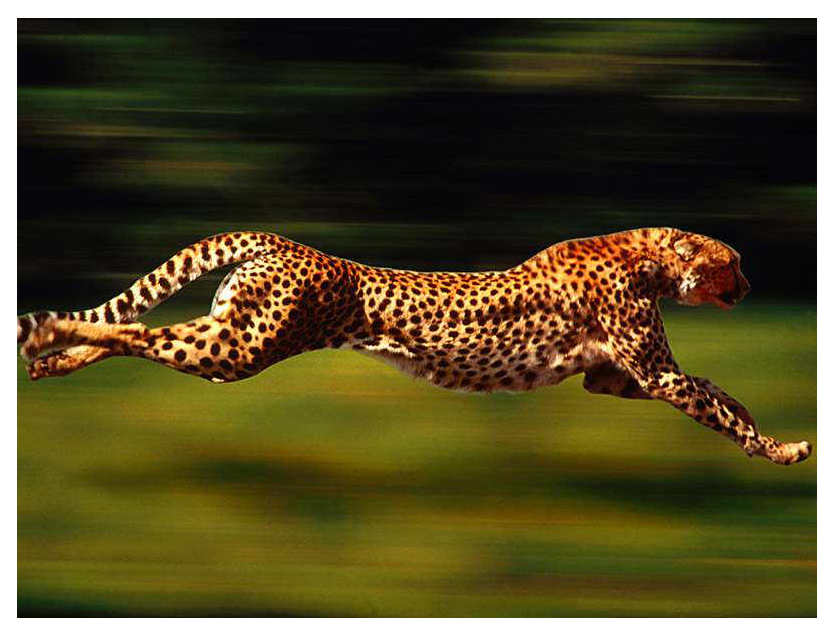
\includegraphics[height=6.0cm]{ambsthermopict/gepard.eps} 
} 
\caption{Life in action.}
\label{nse_people} 
\end{figure}


\begin{figure}[bhpt] 
\centerline{ 
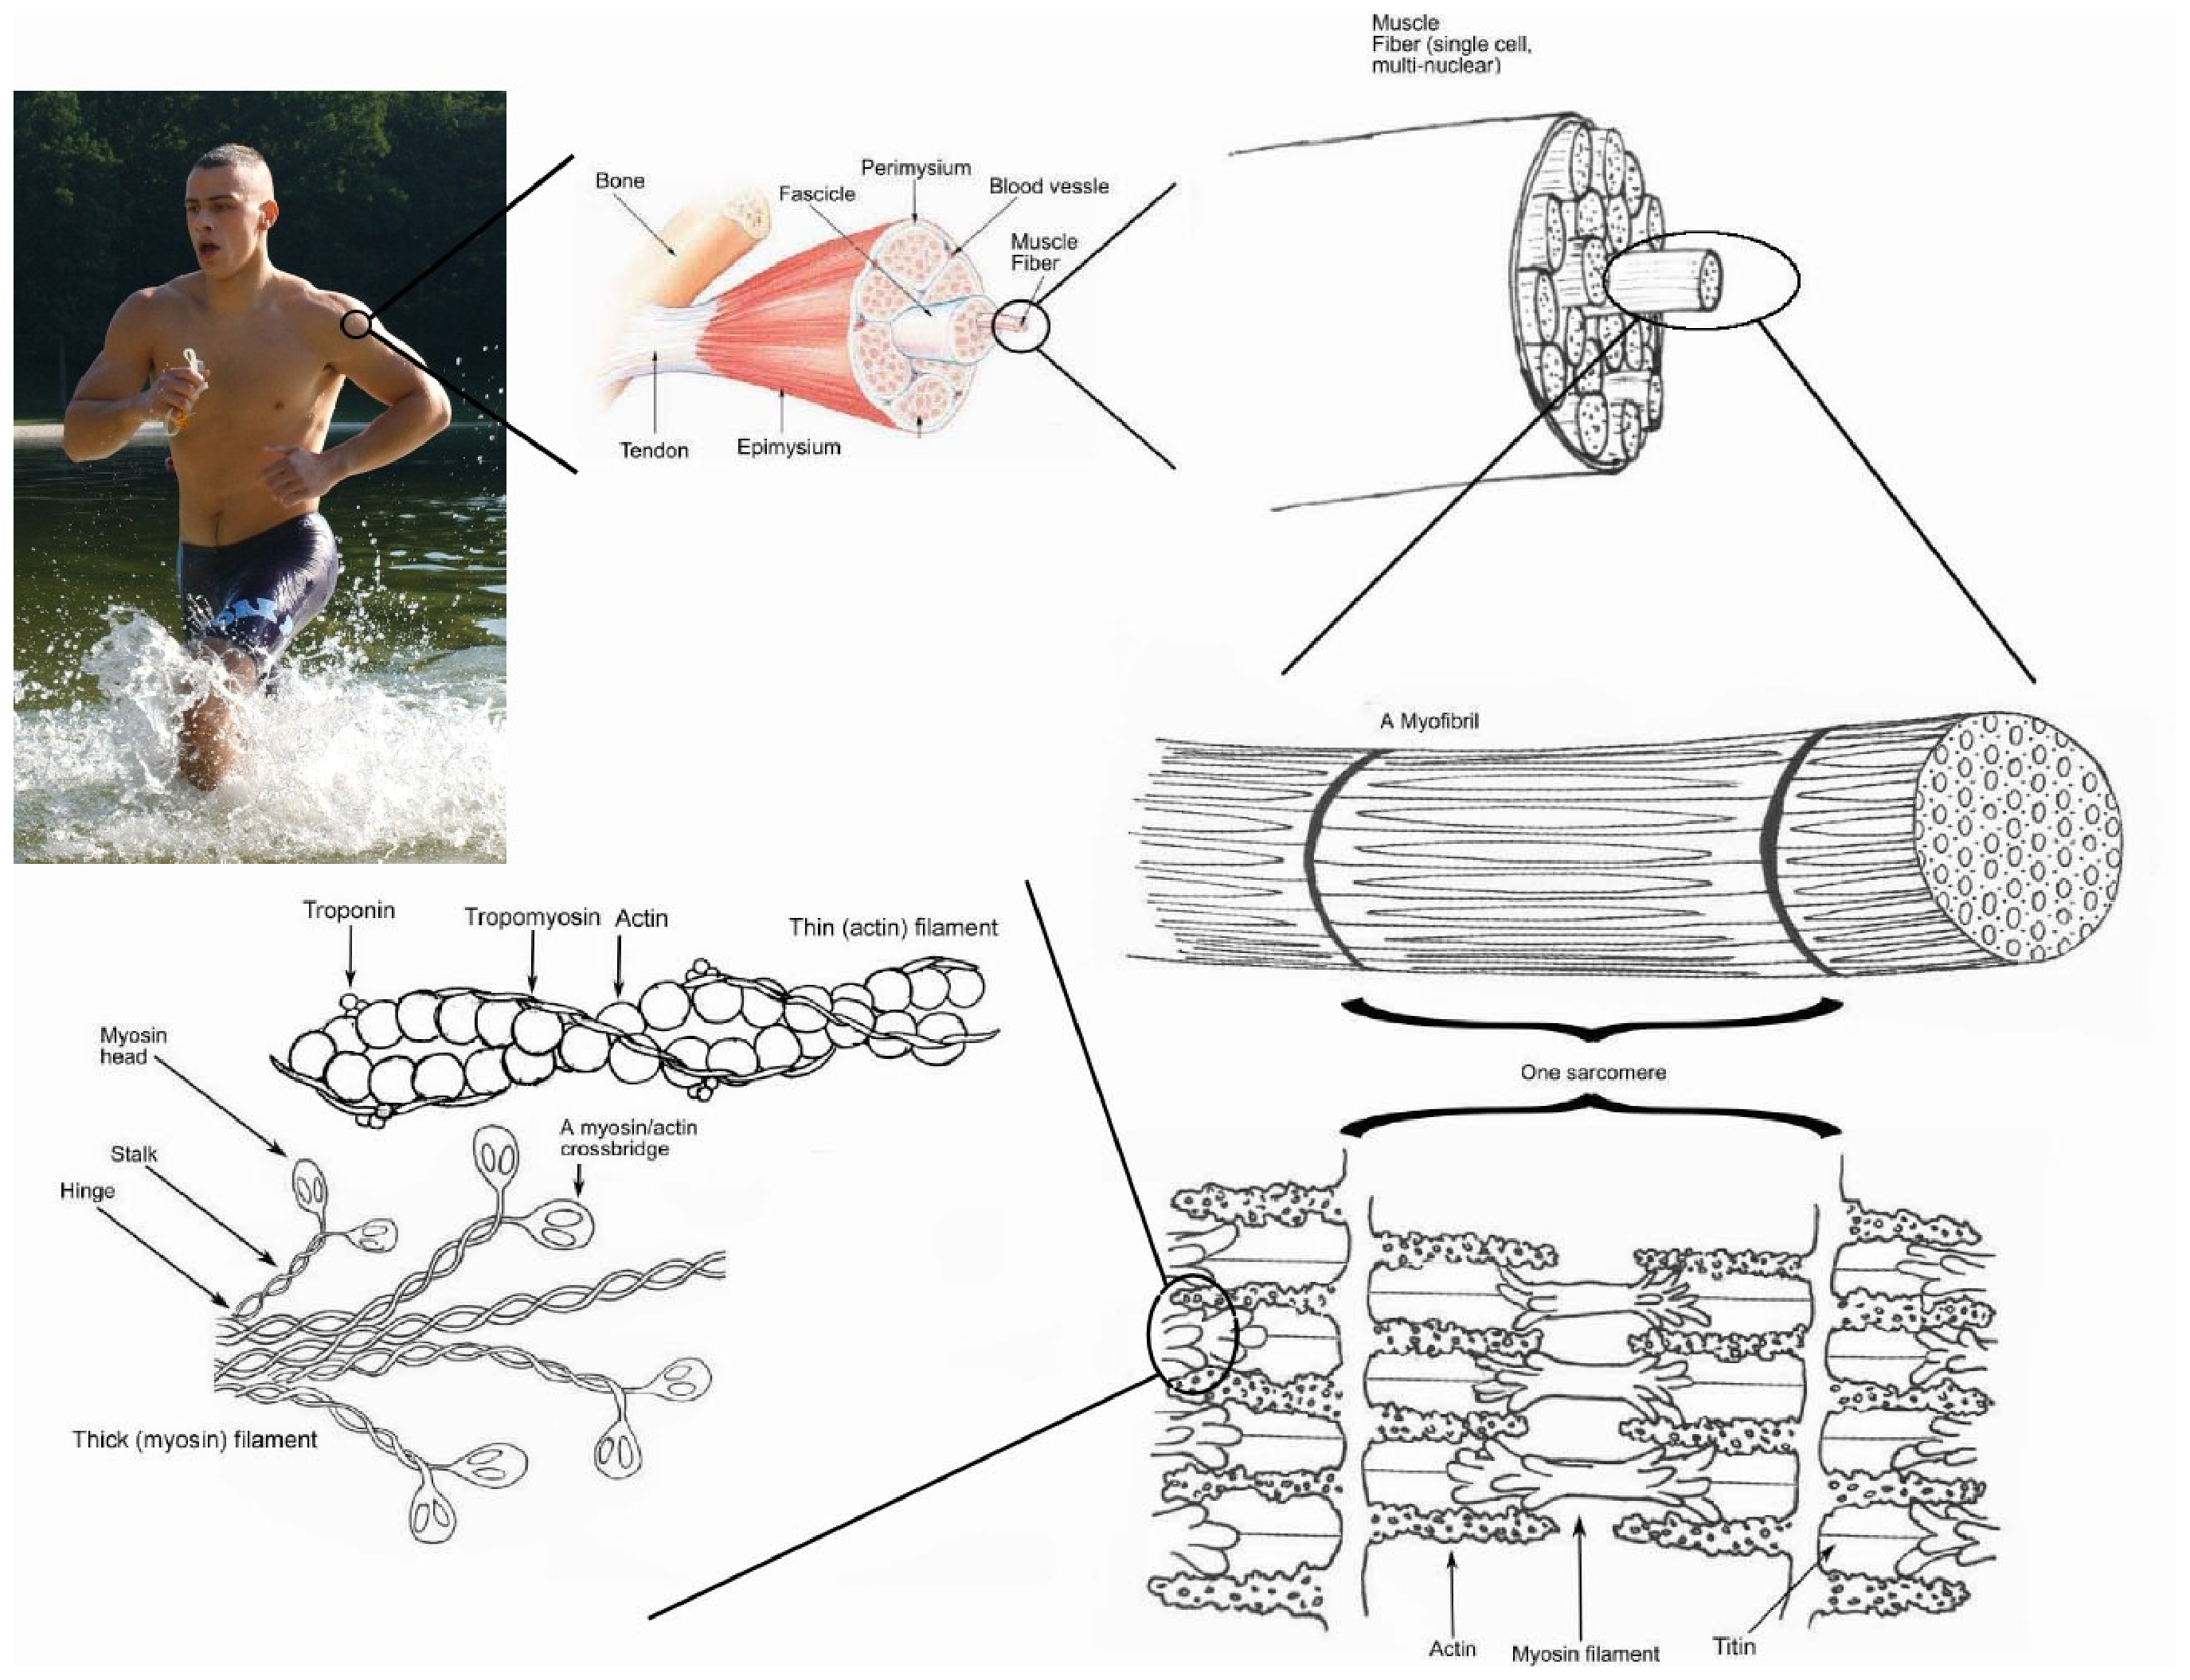
\includegraphics[height=8.5cm]{ambsthermopict/muscle.eps} 
} 
\caption{Muscle contraction by actin-myosin twitch fueled by ATP.}
\label{nse_people} 
\end{figure}




\section{Biology and Life}

Most forms of biological processes build on conversion of
chemical energy into heat and kinetic energy,
and thus ultimately on Solar energy converted to chemical energy 
in the \emph{photo-synthesis}.


\emph{Muscle contraction}  
occurs when a muscle fiber generates tension through
\emph{actin and myosin cross-bridge cycling} shortening the fiber
fueled by \emph{Adanenosine TriPhosphate ATP}.
Locomotion in most higher animals is possible only 
through the repeated contraction of many muscles at the correct times 
controlled by the central nervous system,
the brain and spinal cord. Voluntary muscle contractions 
are initiated in the brain, while the spinal cord initiates involuntary 
reflexes.

The emergence of biological life may naively appear to contradict the 2nd 
Law in its classical form, by creating ordered structures out of disordered, 
while the death of a living organism when order dissolves into disorder,
reflects the classical 2nd Law very well. We shall see that in the
new formulation of the 2nd Law not relying on notions of 
ordered/unordered, there
is nothing (in principle) that prevents ordered structures to develop 
from unordered
(for example in Irak), assuming there is some input of energy (oil). 
%which is kind of a happy message to everybody who is not an extreme pessimist.
%This is one of many indications that
%the classical from of the 2nd Law poses
%difficulties.

\begin{figure}[bhpt] 
\centerline{ 
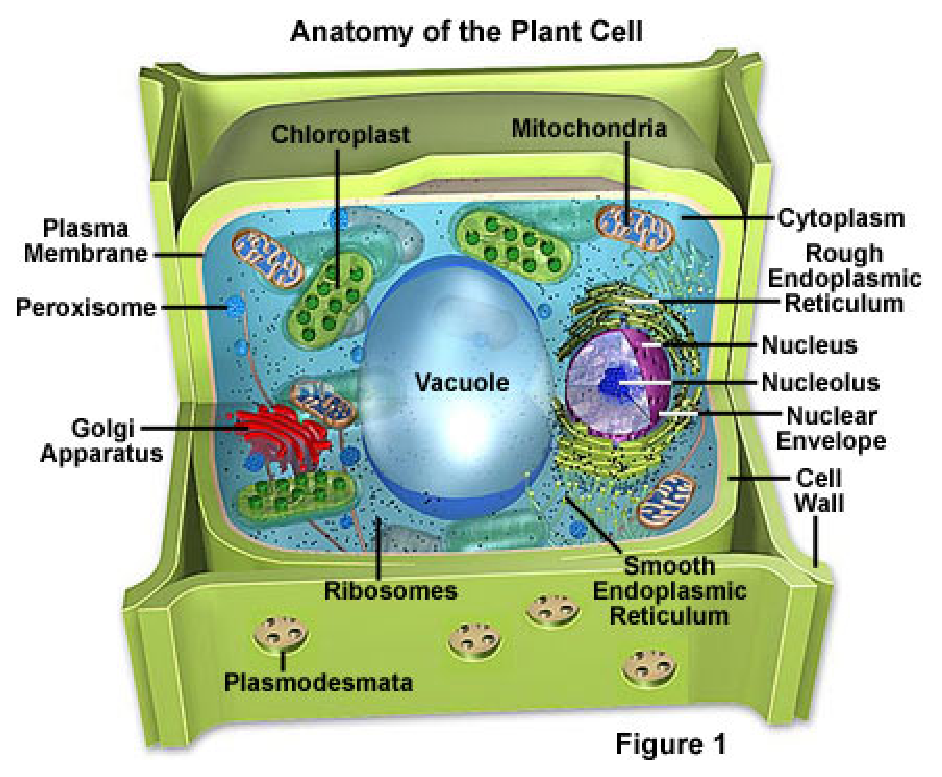
\includegraphics[height=6.0cm]{ambsthermopict/plantcell.eps} 
} 
\caption{Inside a plant cell.}
\label{nse_people} 
\end{figure}


\section{Molecular Biology and Protein Folding}

Biology builds on cell microbiology based on the thermodynamics of
chemical reactions of \emph{protein
synthesis} from amino acid molecules according to
the instructions of \emph{DNA}. Computational thermodynamics of the cell
is becoming an increasingly important tool in medicine and drug design.

%\begin{figure}[bhpt] 
%\centerline{ 
%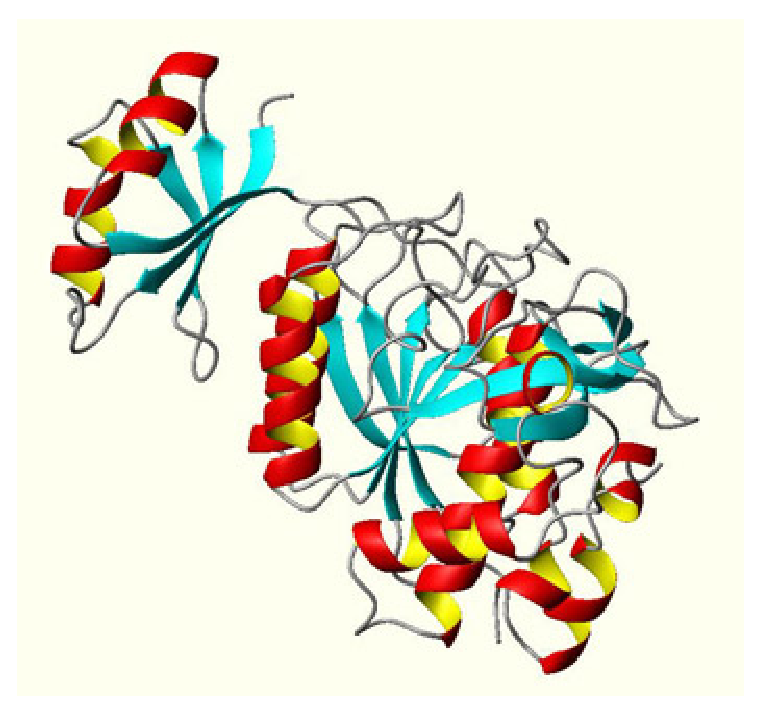
\includegraphics[height=8.0cm]{ambsthermopict/proteinfolding.eps} 
%} 
%\caption{Protein folding}
%\label{nse_people} 
%\end{figure}

%\begin{figure}[bhpt] 
%\centerline{ 
%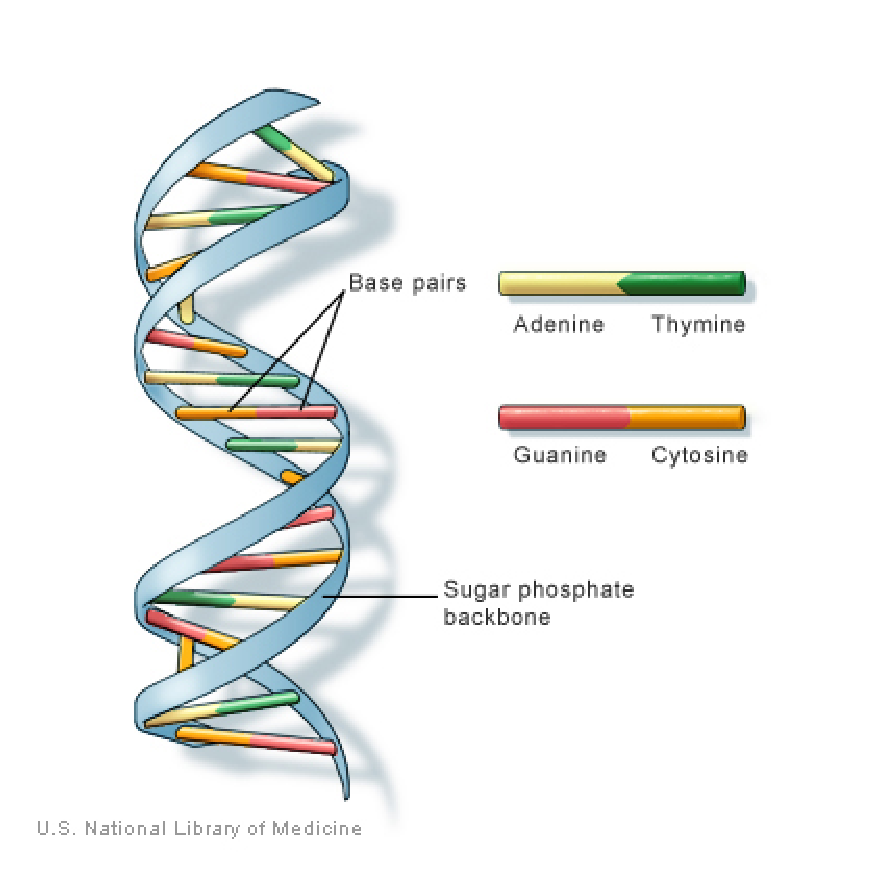
\includegraphics[height=8.0cm]{ambsthermopict/doublehelix.eps} 
%} 
%\caption{The double helix of DNA}
%\label{nse_people} 
%\end{figure}



 
\section{Quantum Physics and Chemistry}

The thermodynamics of chemical reactions and radiation
build on the \emph{quantum mechanics}
of electrons, and the thermodynamics of nuclear reactions build
on quantum electrodynamics of elementary particles. Computational solution
of the equations of quantum mechanics presents a tough challenge, 
because of the richness of the the wave function solution 
with in principle three independent 
space coordinates for each particle (electron) involved. 
Methods
reducing the dimensionality are today routinely used in massive
computations in \emph{quantum chemistry}, and could open to new insights
of the nature of the quarks of elementary particle physics.
%\cite{compquantum}. 

 




\section{Energy Generation and Consumption}

Our \emph{industrial society} is based on production and
consumption of energy in thermodynamic energy conversion processes of 
the form:

\begin{itemize}

\item nuclear/fossile/biological/chemical $\rightarrow$ heat/kinetic/electric, 

\item wind/wave kinetic $\rightarrow$ electric,

\item solar radiation $\rightarrow$ heat/electric.
\item electric $\rightarrow$ heat/kinetic.  
\end{itemize}
In all conversion of energy, minimization of \emph{losses} into useless heat is 
of prime concern, for which computational thermodynamics opens new
possibilities.
\section{Heat Engines and Industrialization}

%The early development of thermodynamics was motivated by the need of 
%understanding the steam engine, underlying the industrialization
%of the Western World in the 19th century.

The industrial society
of the 19th century was built on the use of \emph{steam engines}, and the 
initial motivation to understand thermodynamics came from a need to
increase the efficiency of steam engines for conversion of heat energy to
useful mechanical energy. 
\begin{figure}[bhpt] 
\centerline{ 
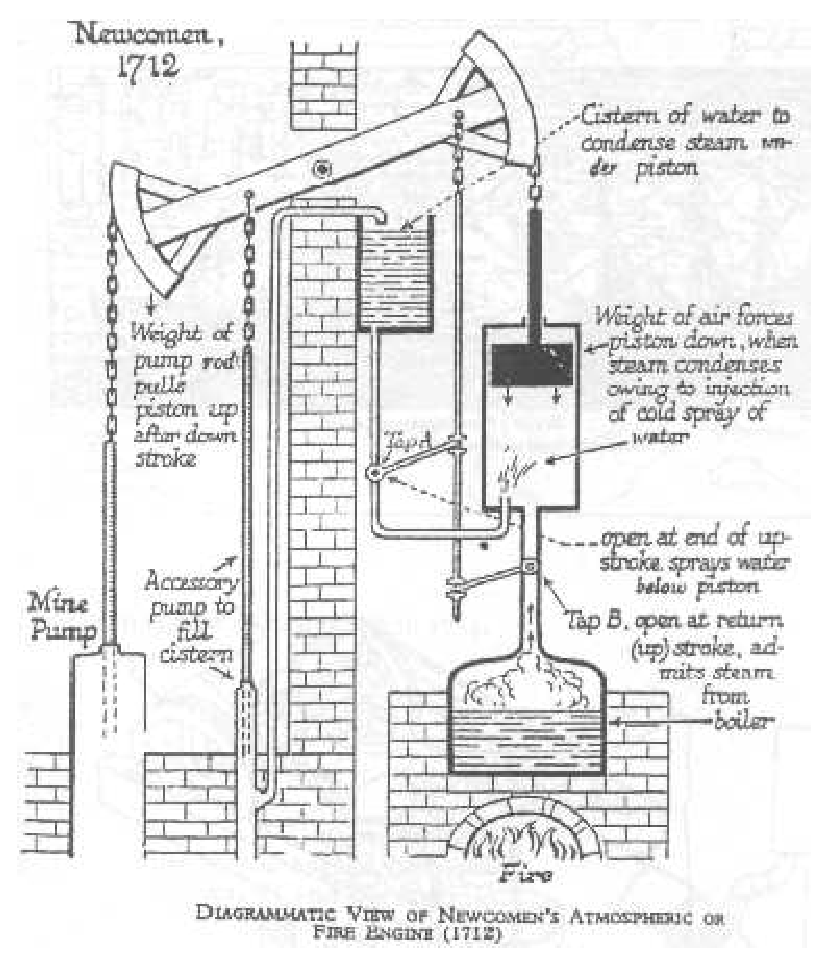
\includegraphics[height=10.0cm]{ambsthermopict/newcdiag.eps} 
} 
\caption{Converting heat to kinetic (mechanical) energy in 1712.}
\label{nse_people} 
\end{figure}  
A steam engine
is a particular form of a 
\emph{heat engine} converting heat to mechanical work in a thermodynamical
process. The modern \emph{combustion engine} in a car 
is a form of heat engine generating kinetic energy
from explosive burning of fuel.
 The efficiency of a heat engine is of 
prime importance, and can be studied by computational thermodynamics.
The necessary \emph{cooling} of a car engine represents 
a loss of energy which is not transformed into useful mechanical work.  

\section{Heat Pumps and Oil Crisis}

The \emph{heat pump} is replacing the increasingly expensive oil
for heating of houses. A heat pump converts low temperature heat energy
from the earth or the air to higher temperature useful heat energy, by
supplying the necessary conversion energy from electricity.
The efficiency is today typically around $2/3$, that is, for $1/3$
unit of electric energy, you get out 1 unit of useful heat energy. 
You can thus reduce your electrical bill by a factor of $3$ by
changing from full electrical heating of your house 
to heating by an efficient heat pump. Of course, it is of interest 
to seek to increase the efficieny even more. Can we reach $99\%$ 
efficiency, and if not why? We will address this question below.

\section{Refrigerators and Urban Civilization}

A \emph{refrigerator} is a form of heat pump taking heat from
the inside of the refrigerator and delivering it to the exterior at
higher temperature. 
The refrigerator is an absolute necessity of modern urban civilization.

The standard design builds on cycling a fluid alternating
between \emph{expansion/evaporation} to gas phase with temperature drop, and 
\emph{compression/condensation} to liquid phase with temperature increase,
with the cold gas in contact with the interior of the refrigerator 
and the warm liquid phase in contact with the exterior.
The cooling process with heat flowing from
cold to hot (contrary to its natural tendency to flow from hot to cold)
is thus maintained by an (electric) \emph{compressor} 
consuming energy.

\begin{figure}[bhpt] 
\centerline{ 
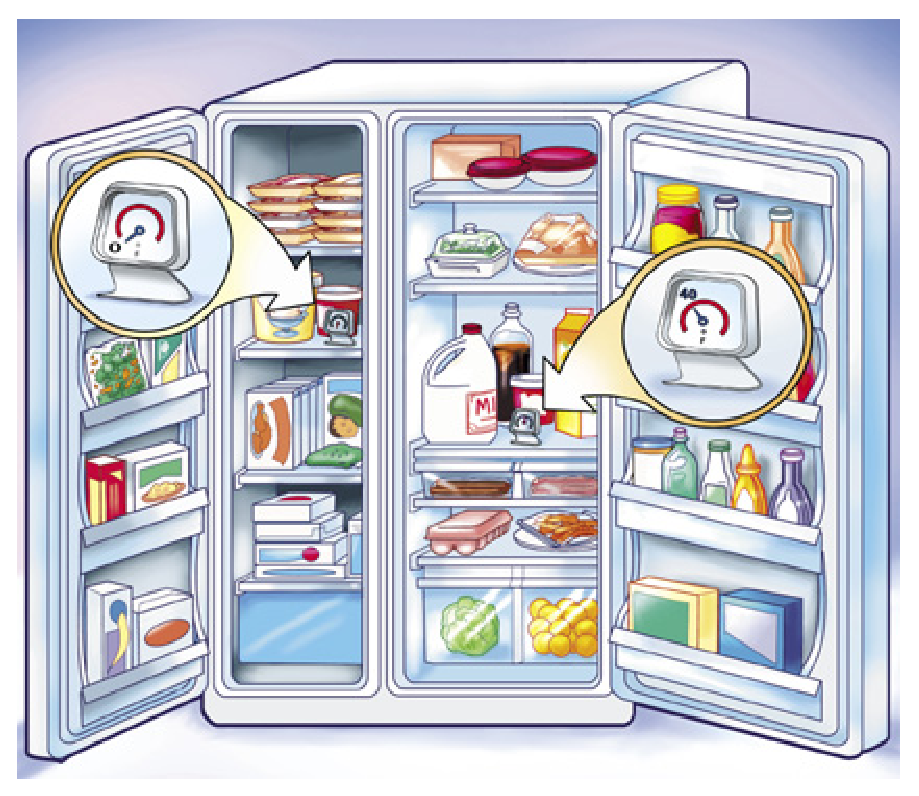
\includegraphics[height=6.0cm]{ambsthermopict/refrigerator.eps} 
} 
\caption{Inside a refrigerator: The principle of preservation of food.}
\label{nse_people} 
\end{figure}




The first design of an \emph{absorption refrigerator}, without compressor and
moving parts and thus silent,
was invented by the two young Swedish
engineering students Carl Munters and Baltzar von
Platen during their class in 
thermodynamics at the Royal Institute of Technology in 1922
(although they slept through the lectures working all night
on their invention).
This invention together with a vacuum cleaner
gave the impetus of the quick expansion of the Electrolux company.
The production of the Munters-Platen refrigerator has 
continued at Motala in Sweden uninterrupted
since 1925 with today a total of 10 million units being produced. 
We hope this book may be useful for young minds of today
for new inventions.


\section{Information and Communication}

\emph{Information theory} was created by Shannon \cite{shannon} in 
the 1940s borrowing the concept of \emph{entropy} from 
\emph{thermodynamics}, with the idea of measuring  
communication channel capacity requirements for different types of information.
Random information would then represent information with
maximal entropy, in principle requiring maximal capacity
(although random information would seem like useless information). 
 
Alternatively, one can view communication of information as a 
thermodynamic flow with the heat energy
representing loss or destruction of information during the communication.
More generally, not only creation but also destruction 
of information represent fundamental aspects of 
physical and biological processes.

\begin{figure}[bhpt] 
\centerline{ 
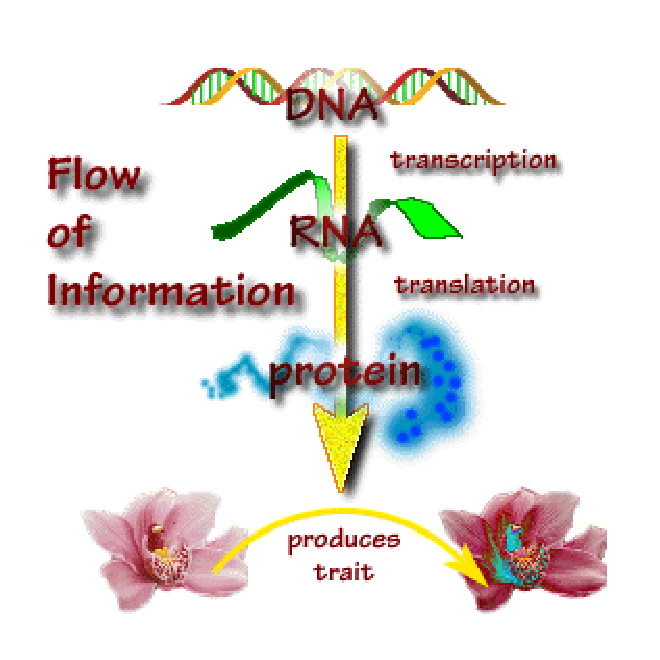
\includegraphics[height=6.0cm]{ambsthermopict/GPFlowInfo.eps} 
} 
\caption{Flow of information in a flower.}
\label{nse_people} 
\end{figure}



\section{Economy and Welfare}

One can also view an evolving economy as a 
thermodynamic flow process transforming resources into utilities.
In (a free) economy turbulent dissipation could be viewed as a measure
of necessary losses during the process, in the form of interest rates,
taxes, bribes, 
thefts, which cannot (fully) be avoided. The flow of the World economy 
represents a complex process of prime importance to all of us.
An economist with (some) understanding of the process can be raised to 
fame and fortune.  

\begin{figure}[bhpt] 
\centerline{ 
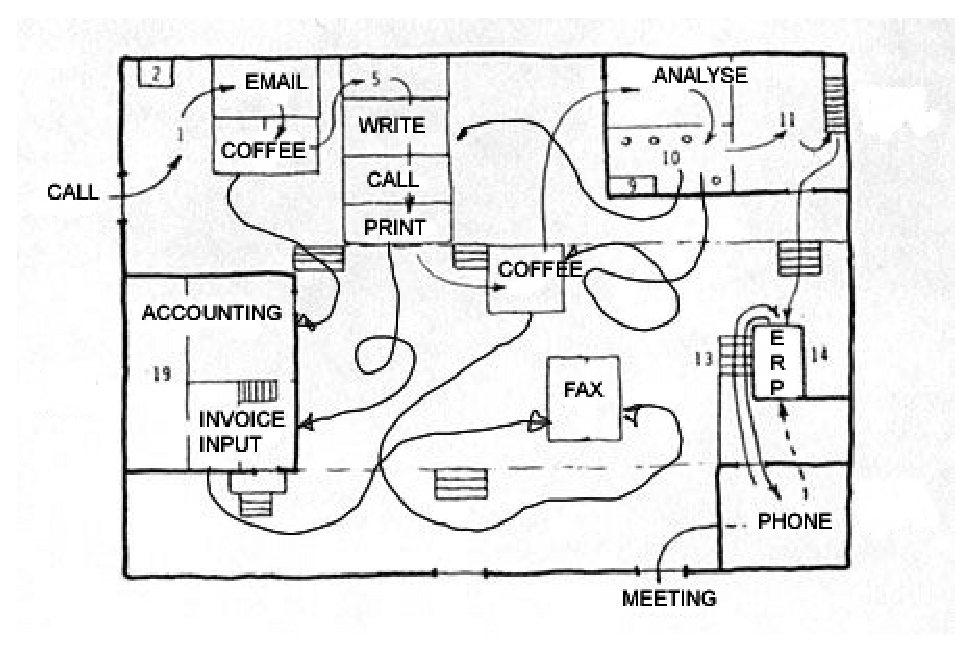
\includegraphics[height=6.0cm]{ambsthermopict/brainshopflow.eps} 
} 
\caption{Flow of information in an office of the last century.}
\label{nse_people} 
\end{figure}

\section{Emergence: A New Approach to Physics}

Ilya Prigogine received the Nobel Prize in Chemistry in 1977
for his work on \emph{non-equlibrium thermodynamics} proposing
a new (statistical) approach to the 2nd Law
allowing ordered structures to develop from non-ordered, see  
%\hyperref[ilyaworld]{Fig. \ref{ilyaworld}} and \ref{ilya}.
Fig. \ref{ilyaworld} and \ref{ilya}.
Even if Prigogine did not convince the physics
community at large, he at least showed the severe short-coming 
of the classical 2nd Law seemingly preventing order from
develping from chaos.

\emph{Emergence} is the process of complex pattern formation
from more basic constituent parts or ``particles'', that is the formation
of order out of chaos. Turbulence shows phenomena of both emergence
and featureless chaos, none of which can be understood by considering only
a single fluid particle, only by considering the interaction of many.
The (new) 2nd Law expresses a collective behavior of many 
fluid particles to form turbulent flow with an 
irreversible transfer of large scale kinetic energy to 
heat energy. Thus thermodynamics
naturally connects to the new approach to physics 
based on emergence, which is now
developing (emerging) 
with input from e.g. 1988 Nobel Laurate Robert Laughlin \cite{laughlin}, 
and which is
radically different from the \emph{reductionist} approach of elementary
particle physics completely dominating the scene since the 
birth of quantum mechanics in the beginning of the last century.

Since emergence concerns the interaction of many particles, analytical
methods fall short (which lies behind the reductionist
obsession with a single particle
hopefully allowing analytical mathematical description),
while computational methods open new possiblities of simulating
emergent and turbulent phenomena, as is shown in this book.


\begin{figure}[bhpt] 
\centerline{ 
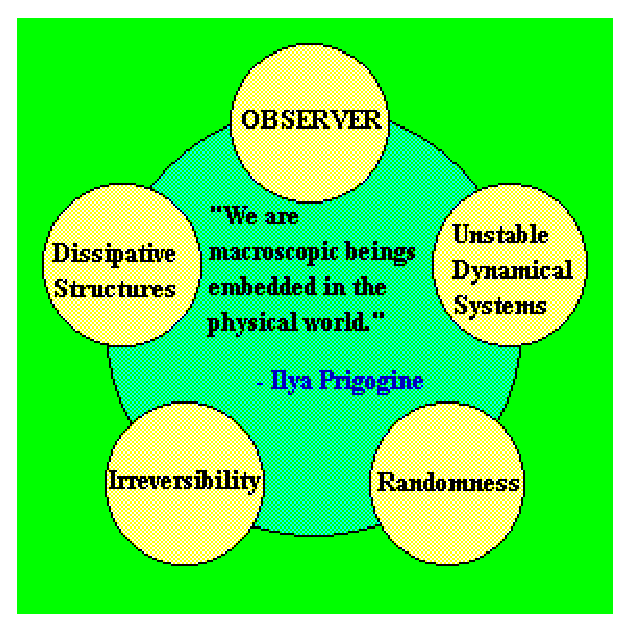
\includegraphics[height=8.0cm]{ambsthermopict/ilyaflow.eps} 
} 
\caption{The World according to Ilya Prigogine.}
\label{ilyaworld} 
\end{figure}\begin{figure}[bhpt] 
\centerline{ 
\includegraphics[height=8.0cm]{ambsthermopict/prigogine.eps} 
} 
\caption{Ilya Prigogine receiving the Nobel Prize in Chemistry
in 1977 from the hands of King Karl XVI Gustav.}
\label{ilya} 
\end{figure}

\section{The Battle between Growth and Decay}

We shall see that turbulent flow and thus thermodynamics (the World)  
can be viewed as a battle between a growth process of \emph{differentiation
by advection} and a decay process of \emph{mixing by diffusion} according
to:
\begin{itemize}
\item \emph{growth: increase difference-differentiate-separate: advection}
\item \emph{decay: decreasse difference--uniformize-mix: diffusion.}
\end{itemize} 
The classical 2nd Law captures the diffusion process with mixing
and decreasing difference. But it does not capture the 
advection process allowing increasing difference and separation,
which is a severe short-coming. The new 2nd Law captures
both processes. In the thermodynamics of Prigogine the two processes are
represented  by ``Unstable Dynamical Systems'' and ``Dissipative Structures'',
but Prigogine sticks to ``Randomness'', see Fig. \ref{ilyaworld}.


\section{Physics: Flow of Information: Computation}

The basic idea of this book 
is to view thermodynamics as a form of 
analog computation, which can be simulated by digital computation. 
Both analog physics and digital computation can be seen as  
flows of information reflecting the flow of mass, momentum and 
energy in a physical system and the flow of digits from input to output in the
execution of a subroutine of the computational code.

For a computer programmer the information flow is 
represented in the flow chart of a computer code, which
is essential for the understanding of the code. 
Likewise, a flow chart of the analog computation 
of a physical process can help the physicist 
to understanding.



 
\section{Thermodynamics as a ``Best of  Worlds''}

The above survey indicates that thermodynamics 
is a fundamental part of science and
technology and thus serves a very important role in our society.
Thermodynamics is maybe the scientific field closest to 
Leibniz' definition of a \emph{Best of Worlds}
as a world, which is richest in variation of ordered complex
structures or emergence, such as different forms of life and conscience,
while being governed by simplest possible principles or laws.



\small
\begin{quote}I say that I am strongly inclined to believe that heat is of 
the same kind, and that material things which make us hot and feel hot 
(such as we call by the general name \emph{fire} are a multitude of tiny 
corpuscles of such and such a shape, and moving at such and such a speed. 
When they meet our bodies, they penetrate them with their extreme subtlety, 
and the way they touch our substance as they pass through it is sensed by 
us as the affection we call ``heat''. 
It is pleasant or unpleasant in 
proportion to the number and speed of the particles as they prick and 
penetrate it. This penetration is pleasant if it is beneficial to our 
insensible vital functions, and unpleasant when it causes too much of a 
separation and dissolution of our substance. (Galieo in \emph{The Assayer}, 
1623)
\end{quote}
\normalsize




